\chapter{Conclusions and Future Works} \label{chap:conclu}
Throughout this thesis, we have researched and analysed reconfiguration problems by starting with the Nondeterministic Constraint Logic
which seems to be the go-to reduction in order to prove $\PSPACE$-hardness results. More specifically, we focused on the alternative
formulation of NCL and detailed the $\PSPACE$-completeness result of the sliding token problem. We then showed that the labelled variant of the
SLIDING TOKEN problem is also $\PSPACE$-complete. This latter result was then used to establish the complexity result of the Exact Cover merge
and split reconfiguration problem which was then used to prove the hardness of the $k$-move Subset sum reconfiguration problem for $k = 3$.
As a contribution to this part, we provided detailed explanatory examples and clarifications to complement the proof.
Every reconfiguration problems we encountered during our journey to the completion of this thesis is summed in fig \ref{fig:conclusion}.

\begin{figure}[H]
    \begin{center}
        \begin{scaletikzpicturetowidth}{\textwidth}
            \begin{tikzpicture}[scale=0.8]
                \node (1) at (0,0) [draw, rounded rectangle, align=center] {CONFIGURATION-TO-EDGE\\for restricted NCL};
                \node (2)  [below left=of 1, draw, rounded rectangle, align=center] {SLIDING-TOKEN\\problem};
                \node (3)  [below right=of 1, draw, rounded rectangle, align=center] {Labelled sliding token\\problem};
                \node (4) [below=of 3, draw, rounded rectangle, align=center] {Exact cover split and merge\\ reconfiguration problem};
                \node (5) [below=of 4, draw, rounded rectangle, align=center] {$k$-move Subset sum\\reconfiguration problem};

                \draw[->]  (1) to node [auto] {$\leq{p}$} (2);
                \draw[->]  (1) to node [auto] {$\leq{p}$} (3);
                \draw[->]  (3) to node [auto] {$\leq{p}$} (4);
                \draw[->]  (4) to node [auto] {$\leq{p}$} (5);
            \end{tikzpicture}
        \end{scaletikzpicturetowidth}
    \end{center}
    \caption{$\PSPACE$-complete problems encountered and their relationship.}\label{fig:conclusion}
\end{figure}

%------------------------************************* Future works **********************------------------------

\section{Future works}

\subsection{SLIDING TOKENS problem}
Given a SLIDING TOKENS instance and two configurations $C_1$ and $C_2$, there may be several reconfiguration sequences to transform the given
initial configuration $C_1$ into $C_2$ (see figures \ref{fig:sequence1} and \ref{fig:sequence2}). Thus, the question of finding the
Shortest reconfiguration path in the SLIDING TOKENS problem naturally arised.


%-------------------------------------------- shortest 1 --------------------------------------------
\begin{figure}[H]
    \centering
    \begin{subfigure}[b]{0.4\textwidth}
        \begin{scaletikzpicturetowidth}{\textwidth}
            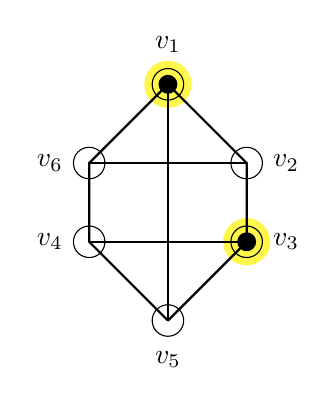
\begin{tikzpicture}[scale=1]
                \def\ver{0.12} %size of a vertex
                \def\xa{1}
                \def\ya{5}
                % highlight change
                \draw[fill=yellow, opacity=.7, draw=none] (\xa,\ya+3)  circle (0.3cm); % v1 ;
                \draw[fill=yellow, opacity=.7, draw=none] (\xa+1,\ya+1)  circle (0.3cm); % v3 ;

                %nodes
                \draw (\xa,\ya) circle (0.2cm);       % v5
                \draw (\xa+1,\ya+1) circle (0.2cm);   % v3
                \draw (\xa+1,\ya+2) circle (0.2cm);   % v2
                \draw (\xa,\ya+3) circle (0.2cm);     % v1
                \draw (\xa-1,\ya+2) circle (0.2cm);   % v6
                \draw (\xa-1,\ya+1) circle (0.2cm);   % v4

                %labels
                \node (1) at (\xa,\ya+3.5) {$v_1$};     % v1
                \node (2) at (\xa+1.5,\ya+2) {$v_2$};   % v2
                \node (3) at (\xa+1.5,\ya+1) {$v_3$};   % v3
                \node (5) at (\xa,\ya-0.5) {$v_5$};     % v5
                \node (4) at (\xa-1.5,\ya+1) {$v_4$};   % v4
                \node (6) at (\xa-1.5,\ya+2) {$v_6$};   % v6

                %token
                \path[fill] (\xa,\ya+3) circle (\ver);   % v1
                \path[fill] (\xa+1,\ya+1) circle (\ver);   % v3

                %edges
                \draw[thick] (\xa,\ya)--(\xa+1,\ya+1)--(\xa+1,\ya+2)--(\xa,\ya+3)--(\xa-1,\ya+2)--(\xa-1,\ya+1)--(\xa,\ya) ; % contour
                \draw[thick] (\xa,\ya)--(\xa,\ya+3) ;       % v5 - v1
                \draw[thick] (\xa+1,\ya+1)--(\xa-1,\ya+1) ; % v3 - v4
                \draw[thick] (\xa+1,\ya+2)--(\xa-1,\ya+2) ; % v2 - v6
            \end{tikzpicture}
        \end{scaletikzpicturetowidth}
        \caption{Initial Independent Set $I_1 = \{v_1, v_3\}$}
        \label{fig:s11}
    \end{subfigure}
    \begin{subfigure}[b]{0.4\textwidth}
        \begin{scaletikzpicturetowidth}{\textwidth}
            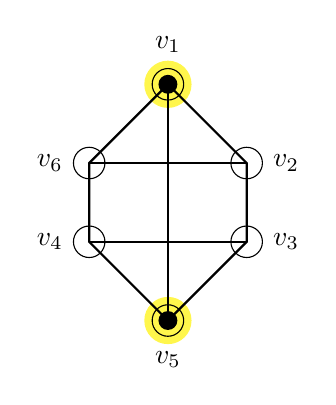
\begin{tikzpicture}[scale=1]
                \def\ver{0.12} %size of a vertex
                \def\xa{1}
                \def\ya{5}
                % highlight change
                \draw[fill=yellow, opacity=.7, draw=none] (\xa,\ya+3)  circle (0.3cm); % v1 ;
                \draw[fill=yellow, opacity=.7, draw=none] (\xa,\ya)  circle (0.3cm); % v5 ;

                %nodes
                \draw (\xa,\ya) circle (0.2cm);       % v5
                \draw (\xa+1,\ya+1) circle (0.2cm);   % v3
                \draw (\xa+1,\ya+2) circle (0.2cm);   % v2
                \draw (\xa,\ya+3) circle (0.2cm);     % v1
                \draw (\xa-1,\ya+2) circle (0.2cm);   % v6
                \draw (\xa-1,\ya+1) circle (0.2cm);   % v4

                %labels
                \node (1) at (\xa,\ya+3.5) {$v_1$};     % v1
                \node (2) at (\xa+1.5,\ya+2) {$v_2$};   % v2
                \node (3) at (\xa+1.5,\ya+1) {$v_3$};   % v3
                \node (5) at (\xa,\ya-0.5) {$v_5$};     % v5
                \node (4) at (\xa-1.5,\ya+1) {$v_4$};   % v4
                \node (6) at (\xa-1.5,\ya+2) {$v_6$};   % v6

                %token
                \path[fill] (\xa,\ya+3) circle (\ver);   % v1
                \path[fill] (\xa,\ya) circle (\ver);     % v5

                %edges
                \draw[thick] (\xa,\ya)--(\xa+1,\ya+1)--(\xa+1,\ya+2)--(\xa,\ya+3)--(\xa-1,\ya+2)--(\xa-1,\ya+1)--(\xa,\ya) ; % contour
                \draw[thick] (\xa,\ya)--(\xa,\ya+3) ;       % v5 - v1
                \draw[thick] (\xa+1,\ya+1)--(\xa-1,\ya+1) ; % v3 - v4
                \draw[thick] (\xa+1,\ya+2)--(\xa-1,\ya+2) ; % v2 - v6
            \end{tikzpicture}
        \end{scaletikzpicturetowidth}
        \caption{Intermediate Independent Set}
        \label{fig:s12}
    \end{subfigure}
    \begin{subfigure}[b]{0.4\textwidth}
        \begin{scaletikzpicturetowidth}{\textwidth}
            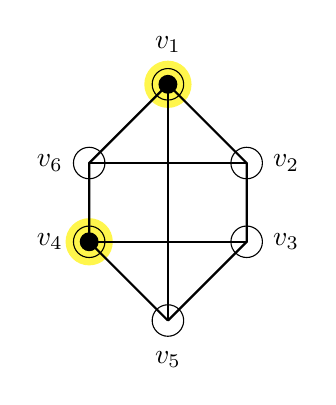
\begin{tikzpicture}[scale=1]
                \def\ver{0.12} %size of a vertex
                \def\xa{1}
                \def\ya{5}
                % highlight change
                \draw[fill=yellow, opacity=.7, draw=none] (\xa,\ya+3)  circle (0.3cm); % v1 ;
                \draw[fill=yellow, opacity=.7, draw=none] (\xa-1,\ya+1) circle (0.3cm); % v4 ;

                %nodes
                \draw (\xa,\ya) circle (0.2cm);       % v5
                \draw (\xa+1,\ya+1) circle (0.2cm);   % v3
                \draw (\xa+1,\ya+2) circle (0.2cm);   % v2
                \draw (\xa,\ya+3) circle (0.2cm);     % v1
                \draw (\xa-1,\ya+2) circle (0.2cm);   % v6
                \draw (\xa-1,\ya+1) circle (0.2cm);   % v4

                %labels
                \node (1) at (\xa,\ya+3.5) {$v_1$};     % v1
                \node (2) at (\xa+1.5,\ya+2) {$v_2$};   % v2
                \node (3) at (\xa+1.5,\ya+1) {$v_3$};   % v3
                \node (5) at (\xa,\ya-0.5) {$v_5$};     % v5
                \node (4) at (\xa-1.5,\ya+1) {$v_4$};   % v4
                \node (6) at (\xa-1.5,\ya+2) {$v_6$};   % v6

                %token
                \path[fill] (\xa,\ya+3) circle (\ver);   % v1
                \path[fill] (\xa-1,\ya+1) circle (\ver); % v4

                %edges
                \draw[thick] (\xa,\ya)--(\xa+1,\ya+1)--(\xa+1,\ya+2)--(\xa,\ya+3)--(\xa-1,\ya+2)--(\xa-1,\ya+1)--(\xa,\ya) ; % contour
                \draw[thick] (\xa,\ya)--(\xa,\ya+3) ;       % v5 - v1
                \draw[thick] (\xa+1,\ya+1)--(\xa-1,\ya+1) ; % v3 - v4
                \draw[thick] (\xa+1,\ya+2)--(\xa-1,\ya+2) ; % v2 - v6
            \end{tikzpicture}
        \end{scaletikzpicturetowidth}
        \caption{Target Independent Set $I_2 = \{v_2, v_4\}$}
        \label{fig:s13}
    \end{subfigure}
    \begin{subfigure}[b]{0.4\textwidth}
        \begin{scaletikzpicturetowidth}{\textwidth}
            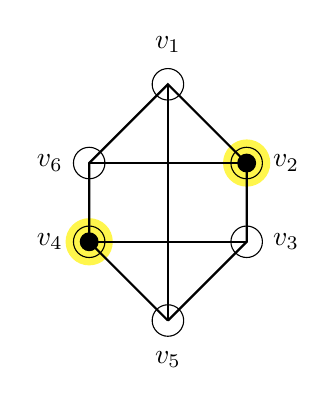
\begin{tikzpicture}[scale=1]
                \def\ver{0.12} %size of a vertex
                \def\xa{1}
                \def\ya{5}
                % highlight change
                \draw[fill=yellow, opacity=.7, draw=none] (\xa+1,\ya+2) circle (0.3cm); % v2 ;
                \draw[fill=yellow, opacity=.7, draw=none] (\xa-1,\ya+1) circle (0.3cm); % v4 ;

                %nodes
                \draw (\xa,\ya) circle (0.2cm);       % v5
                \draw (\xa+1,\ya+1) circle (0.2cm);   % v3
                \draw (\xa+1,\ya+2) circle (0.2cm);   % v2
                \draw (\xa,\ya+3) circle (0.2cm);     % v1
                \draw (\xa-1,\ya+2) circle (0.2cm);   % v6
                \draw (\xa-1,\ya+1) circle (0.2cm);   % v4

                %labels
                \node (1) at (\xa,\ya+3.5) {$v_1$};     % v1
                \node (2) at (\xa+1.5,\ya+2) {$v_2$};   % v2
                \node (3) at (\xa+1.5,\ya+1) {$v_3$};   % v3
                \node (5) at (\xa,\ya-0.5) {$v_5$};     % v5
                \node (4) at (\xa-1.5,\ya+1) {$v_4$};   % v4
                \node (6) at (\xa-1.5,\ya+2) {$v_6$};   % v6

                %token
                \path[fill] (\xa+1,\ya+2) circle (\ver); % v2
                \path[fill] (\xa-1,\ya+1) circle (\ver); % v4

                %edges
                \draw[thick] (\xa,\ya)--(\xa+1,\ya+1)--(\xa+1,\ya+2)--(\xa,\ya+3)--(\xa-1,\ya+2)--(\xa-1,\ya+1)--(\xa,\ya) ; % contour
                \draw[thick] (\xa,\ya)--(\xa,\ya+3) ;       % v5 - v1
                \draw[thick] (\xa+1,\ya+1)--(\xa-1,\ya+1) ; % v3 - v4
                \draw[thick] (\xa+1,\ya+2)--(\xa-1,\ya+2) ; % v2 - v6
            \end{tikzpicture}
        \end{scaletikzpicturetowidth}
        \caption{A $3$-regular graph $G=(V,E)$ and initial independent set $I_1 = \{v_1, v_3\}$}
        \label{fig:s14}
    \end{subfigure}
    \caption{Configuration-to-edge input instance}
    \label{fig:sequence1}
\end{figure}

%-------------------------------------------- shortest 2 --------------------------------------------
\begin{figure}[H]
    \centering
    \begin{subfigure}[b]{0.3\textwidth}
        \begin{scaletikzpicturetowidth}{\textwidth}
            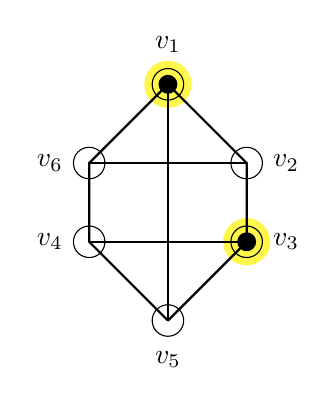
\begin{tikzpicture}[scale=1]
                \def\ver{0.12} %size of a vertex
                \def\xa{1}
                \def\ya{5}
                % highlight change
                \draw[fill=yellow, opacity=.7, draw=none] (\xa,\ya+3)  circle (0.3cm); % v1 ;
                \draw[fill=yellow, opacity=.7, draw=none] (\xa+1,\ya+1)  circle (0.3cm); % v3 ;

                %nodes
                \draw (\xa,\ya) circle (0.2cm);       % v5
                \draw (\xa+1,\ya+1) circle (0.2cm);   % v3
                \draw (\xa+1,\ya+2) circle (0.2cm);   % v2
                \draw (\xa,\ya+3) circle (0.2cm);     % v1
                \draw (\xa-1,\ya+2) circle (0.2cm);   % v6
                \draw (\xa-1,\ya+1) circle (0.2cm);   % v4

                %labels
                \node (1) at (\xa,\ya+3.5) {$v_1$};     % v1
                \node (2) at (\xa+1.5,\ya+2) {$v_2$};   % v2
                \node (3) at (\xa+1.5,\ya+1) {$v_3$};   % v3
                \node (5) at (\xa,\ya-0.5) {$v_5$};     % v5
                \node (4) at (\xa-1.5,\ya+1) {$v_4$};   % v4
                \node (6) at (\xa-1.5,\ya+2) {$v_6$};   % v6

                %token
                \path[fill] (\xa,\ya+3) circle (\ver);   % v1
                \path[fill] (\xa+1,\ya+1) circle (\ver);   % v3

                %edges
                \draw[thick] (\xa,\ya)--(\xa+1,\ya+1)--(\xa+1,\ya+2)--(\xa,\ya+3)--(\xa-1,\ya+2)--(\xa-1,\ya+1)--(\xa,\ya) ; % contour
                \draw[thick] (\xa,\ya)--(\xa,\ya+3) ;       % v5 - v1
                \draw[thick] (\xa+1,\ya+1)--(\xa-1,\ya+1) ; % v3 - v4
                \draw[thick] (\xa+1,\ya+2)--(\xa-1,\ya+2) ; % v2 - v6
            \end{tikzpicture}
        \end{scaletikzpicturetowidth}
        \caption{Initial Independent Set $I_1 = \{v_1, v_3\}$}
        \label{fig:s21}
    \end{subfigure}
    \begin{subfigure}[b]{0.3\textwidth}
        \begin{scaletikzpicturetowidth}{\textwidth}
            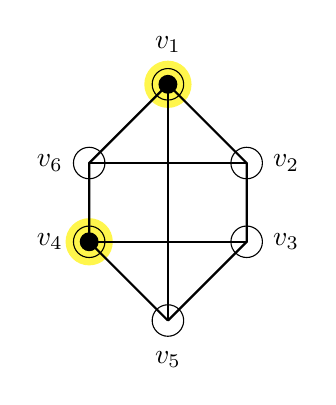
\begin{tikzpicture}[scale=1]
                \def\ver{0.12} %size of a vertex
                \def\xa{1}
                \def\ya{5}
                % highlight change
                \draw[fill=yellow, opacity=.7, draw=none] (\xa,\ya+3)  circle (0.3cm); % v1 ;
                \draw[fill=yellow, opacity=.7, draw=none] (\xa-1,\ya+1)  circle (0.3cm); % v4 ;

                %nodes
                \draw (\xa,\ya) circle (0.2cm);       % v5
                \draw (\xa+1,\ya+1) circle (0.2cm);   % v3
                \draw (\xa+1,\ya+2) circle (0.2cm);   % v2
                \draw (\xa,\ya+3) circle (0.2cm);     % v1
                \draw (\xa-1,\ya+2) circle (0.2cm);   % v6
                \draw (\xa-1,\ya+1) circle (0.2cm);   % v4

                %labels
                \node (1) at (\xa,\ya+3.5) {$v_1$};     % v1
                \node (2) at (\xa+1.5,\ya+2) {$v_2$};   % v2
                \node (3) at (\xa+1.5,\ya+1) {$v_3$};   % v3
                \node (5) at (\xa,\ya-0.5) {$v_5$};     % v5
                \node (4) at (\xa-1.5,\ya+1) {$v_4$};   % v4
                \node (6) at (\xa-1.5,\ya+2) {$v_6$};   % v6

                %token
                \path[fill] (\xa,\ya+3) circle (\ver);   % v1
                \path[fill] (\xa-1,\ya+1) circle (\ver); % v4

                %edges
                \draw[thick] (\xa,\ya)--(\xa+1,\ya+1)--(\xa+1,\ya+2)--(\xa,\ya+3)--(\xa-1,\ya+2)--(\xa-1,\ya+1)--(\xa,\ya) ; % contour
                \draw[thick] (\xa,\ya)--(\xa,\ya+3) ;       % v5 - v1
                \draw[thick] (\xa+1,\ya+1)--(\xa-1,\ya+1) ; % v3 - v4
                \draw[thick] (\xa+1,\ya+2)--(\xa-1,\ya+2) ; % v2 - v6
            \end{tikzpicture}
        \end{scaletikzpicturetowidth}
        \caption{Intermediate Independent Set}
        \label{fig:s22}
    \end{subfigure}
    \begin{subfigure}[b]{0.3\textwidth}
        \begin{scaletikzpicturetowidth}{\textwidth}
            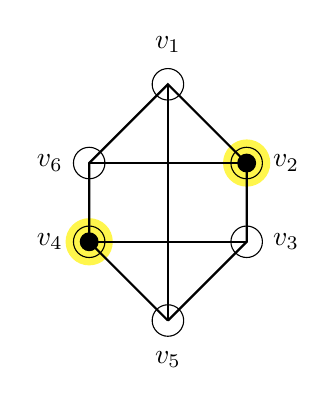
\begin{tikzpicture}[scale=1]
                \def\ver{0.12} %size of a vertex
                \def\xa{1}
                \def\ya{5}
                % highlight change
                \draw[fill=yellow, opacity=.7, draw=none] (\xa+1,\ya+2)  circle (0.3cm); % v2 ;
                \draw[fill=yellow, opacity=.7, draw=none] (\xa-1,\ya+1) circle (0.3cm); % v4 ;

                %nodes
                \draw (\xa,\ya) circle (0.2cm);       % v5
                \draw (\xa+1,\ya+1) circle (0.2cm);   % v3
                \draw (\xa+1,\ya+2) circle (0.2cm);   % v2
                \draw (\xa,\ya+3) circle (0.2cm);     % v1
                \draw (\xa-1,\ya+2) circle (0.2cm);   % v6
                \draw (\xa-1,\ya+1) circle (0.2cm);   % v4

                %labels
                \node (1) at (\xa,\ya+3.5) {$v_1$};     % v1
                \node (2) at (\xa+1.5,\ya+2) {$v_2$};   % v2
                \node (3) at (\xa+1.5,\ya+1) {$v_3$};   % v3
                \node (5) at (\xa,\ya-0.5) {$v_5$};     % v5
                \node (4) at (\xa-1.5,\ya+1) {$v_4$};   % v4
                \node (6) at (\xa-1.5,\ya+2) {$v_6$};   % v6

                %token
                \path[fill] (\xa+1,\ya+2) circle (\ver);   % v2
                \path[fill] (\xa-1,\ya+1) circle (\ver); % v4

                %edges
                \draw[thick] (\xa,\ya)--(\xa+1,\ya+1)--(\xa+1,\ya+2)--(\xa,\ya+3)--(\xa-1,\ya+2)--(\xa-1,\ya+1)--(\xa,\ya) ; % contour
                \draw[thick] (\xa,\ya)--(\xa,\ya+3) ;       % v5 - v1
                \draw[thick] (\xa+1,\ya+1)--(\xa-1,\ya+1) ; % v3 - v4
                \draw[thick] (\xa+1,\ya+2)--(\xa-1,\ya+2) ; % v2 - v6
            \end{tikzpicture}
        \end{scaletikzpicturetowidth}
        \caption{Target Independent Set $I_2 = \{v_2, v_4\}$}
        \label{fig:s23}
    \end{subfigure}
    \caption{Configuration-to-edge input instance}
    \label{fig:sequence2}
\end{figure}

However this question has already been asked by Yamada and Uehara in 2016, defined below and remains open. The difficulty lies in
computing the reconfiguration graph.
\begin{flushleft}
    Shortest Sliding Token [Yamada and Uehara 2016]\\
    \textbf{Instance: } A yes-instance $(G, I, J)$ of Sliding Token, where $I, J$ are independent sets of a graph $G$. \\
    \textbf{Question: } Find a shortest TS-sequence that transforms $I$ into $J$ (and vice versa) \\
\end{flushleft}

On the bright side, in the past years positive results have been established for cographs, interval graphs, caterpillars, trees,
prefect graphs and spider graphs. Those interesting results are summed up below.
\begin{theorem}(Kaminski et al. 2012)
It is $\NP$-complete to decide if there is a TS-sequence having at most $l$ token-slides between two independent sets $I, J$ of a
perfect graph $G$ even when $l$ is polynomial in $|V(G)|$.
\end{theorem}

\begin{theorem}(Kaminski et al. 2012)
Shortest Sliding Token can be solved in linear time for cographs (P4-free graphs).
\end{theorem}

\begin{theorem}(Yamada and Uehara 2016)
Shortest Sliding Token can be solved in polynomial time for proper interval graphs, trivially perfect graphs, and caterpillars.
\end{theorem}

\begin{theorem}(Sugimori, AAAC 2018)
Shortest Sliding Token can be solved in $O(poly(n))$ time when the input graph is a tree on $n$ vertices.
\end{theorem}

\begin{theorem}(Ryuhei Uehara, CIAC 2019)
Shortest Sliding Token can be solved in $O(n^2)$ time when the input graph is a spider (i.e., a tree having exactly one
vertex of degree at least $3$) on $n$ vertices.
\end{theorem}


\subsection{$3$-move SUBSET SUM RECONFIGURATION problem}
Recall that we studied the following problem in chapter \ref{chap:subset-sum-reconf} :
\begin{defn}{($k$-move SUBSET SUM RECONFIGURATION Problem).} Given two solutions $A_1$ and $A_2$ to an instance of the subset sum problem,
can $A_2$ be obtained by repeated $k$-move reconfiguration, beginning with $A_1$, so that all intermediate subsets are also solutions?
\end{defn}

It would be interesting to study the connectivity question of the $k$-move SUBSET SUM RECONFIGURATION problem defined below :
\begin{defn}{($k$-move SUBSET SUM RECONFIGURATION Problem conn).} Given an integer $x$ and a set of integers $S = \{a_1, a_2, \dots, a_n\}$,
let $G(S)$ be the subgraph graph induced by the feasible solutions of $S$ where there is an edge between two vertices
of $G(S)$ iff the symmetric difference is at most $k$. Is $G(S)$ connected ?
\end{defn}

Another question concerns finding an optimal coloring with $k$ colors that is smaller than $23$ for the ECR problem.
